\documentclass[11pt]{article}
\usepackage{ucs}
\usepackage[utf8x]{inputenc}
\usepackage{changepage}
\usepackage{graphicx}
\usepackage{amsmath}
\usepackage{gensymb}
\usepackage{amssymb}
\usepackage{enumerate}
\usepackage{tabularx}
\usepackage{lipsum}
\usepackage{hyperref}
\usepackage{fancyvrb}

\oddsidemargin 0.0in
\evensidemargin 0.0in
\textwidth 6.27in
\headheight 1.0in
\topmargin -0.1in
\headheight 0.0in
\headsep 0.0in
\textheight 9.0in

\usepackage{xcolor}

\setlength\parindent{0pt}

\newenvironment{myenv}{\begin{adjustwidth}{0.4in}{0.4in}}{\end{adjustwidth}}
\renewcommand{\abstractname}{Anotācija}
\renewcommand\refname{Atsauces}



\newcounter{alphnum}
\newenvironment{alphlist}{\begin{list}{(\Alph{alphnum})}{\usecounter{alphnum}\setlength{\leftmargin}{2.5em}} \rm}{\end{list}}


%16.3-6

\makeatletter
\let\saved@bibitem\@bibitem
\makeatother

\usepackage{bibentry}



\begin{document}
\thispagestyle{empty}


\begin{center}
{\Large C++ Exercise 7: Aliens}
\end{center}

{\bf Deadline:} Monday, November 9, 2020 by 23:59:59 EET Timezone.\\ 
{\bf How to submit:} Check your code into your GitHub repository, 
the default {\tt master} branch, 
tag it as {\tt ex07submit} (all lowercase, no dashes).\\
{\bf Grading:} This exercise is worth 100\textperthousand (or $10\%$) of the total grade.\\
{\bf Objectives:} Using pointers, arrays, user-defined classes (but no external libraries like STL 
or Boost) complete the node traversal exercise described below: Read input from STDIN, write output
to STDOUT and report error conditions, if input data has inconsistencies.
{\bf Performance targets:} RAM Memory: 4 MiB. Run-Time on a single input file: 0.1 seconds.\\ 
If your program is correct, but not very efficient, you can still 
get most of the credit (about $70\%$ of the testcases will be small: no more than $100$ nodes of the input data). 
But the performance targets should guide you against choosing some outrageously inefficient algorithms.
{\bf UML Class Design:} During the first week we suggest that you develop 
a class design (preferrably as a UML diagram or, maybe, a set of CPP header files) showing 
the function prototypes that you will use. And some testcases (Check2 or anything else) to test these functions. 
It should be submitted by {\bf November 2} (a separate folder in ORTUS). 
During the second week you can write all the code to implement this class design (you can make changes, 
if you find out that you do not like your class design).  



\vspace{20pt}
{\bf Description}

In 2020 humans sent an autonomous robot {\em Perseverance} to Mars. 
(The goals were explained in their press-release as follows: 
"The program's ongoing series of missions is helping us answer key questions 
about the potential for life on Mars. While previous missions have helped us 
look for signs of habitable conditions in ancient times, 
{\em Perseverance} will take it one step further by searching for signs of past microbial life itself.")
Soon {\em Perseverance} noticed various signs of life on Mars. They took images of green creatures 
who could change their location. After trying to hide for some time, the creatures (subsequently called {\em aliens}) 
started to communicate with our civilization.

To address culture differences and avoid misunderstandings, earthlings became interested 
in the everyday life of aliens. As they found out, aliens have asexual reproduction: 
every alien can have no more than two children. Every child is either left-handed or right-handed. 
Additionally, if an alien has two children, they are necessarily of different types: one of them is left-handed, 
and the other one is right-handed. Reproduction can happen soon after birth, 
many generations can live simultaneously. Since aliens have very large families, 
every alien maintains close relationship with its {\em favourite relatives} (every alien 
has up to $2$ such relatives). 

Earthlings wanted to find out, how to identify the two (or fewer) favorite relatives for the given alien. 
First, we pick some alien without living parent. Then draw the family tree 
(the tree of parent-child relationships with the given alien as the root).  
Every alien in this family tree has two favorite relatives immediately preceding him and 
immediately following him in the {\em inorder} DFS traversal of that tree. 
Left-handed aliens are shown to the left of their parent, the right-hinded ones - to the right. 

Your task is to build an efficient program that receives the genealogy data for 
one or more family trees, and it finds the two favorite relative aliens for any given alien upon 
receiving a query.

It is known that no more than $10\,000$ aliens are currently alive. 
Every alien has a unique number $[1..10\,000]$.


\vspace{20pt}
{\bf Input}

We add nodes one at a time. Commands can come at any order 
(but if we add a child, its parent must be added \textendash{} 
otherwise it should be reported as an error). 
In-between the commands (that gradually build a ``forest'' of one or more trees) we 
can add query commands to find the {\em favorite relatives} for a given node 
in the tree that has been built so far. 

The input file contains one of these five commands that build 
a collection of genealogy trees:

\begin{enumerate}
\item Specify a {\em Top living ancestor} of an alien family tree (it has no living parents). 
\item Specify the {\em Left-handed child} for a parent. 
\item Specify the {\em right-handed child} for a parent. 
\item Query for the favorite relatives of a given alien. 
\item Finish your work. 
\end{enumerate}

The syntax for all these commands looks like this:

\begin{verbatim}
T Ancestor
...
L Parent Child
...
R Parent Child
...
? Alien
...
F
\end{verbatim}

\begin{itemize}
\item {\tt Ancestor} is a number for an alien that is a {\em top living ancestor} of some genealogy tree. 
({\tt Ancestor} may stay the only node in his tree; then both his favorite relatives are nonexistent). 
\item {\tt L} is the command to specify the left-handed {\tt Child} for a {\tt Parent}. 
\item {\tt R} is the command to specify the right-handed child for a parent.
\item In the query command {\tt Alien} is the alien identificator in the request to find the favorite relatives. 
\item Any identificator for a an alien ({\tt Ancestor}, {\tt Parent}, {\tt Child}, {\tt Alien}) 
is an integer number from the interval $[1;\,10\,000])$
\end{itemize}

The input data is valid - regarding the format and the limitations defined above. 
Some tree editing commands may refer to nodes that cannot be inserted (such commands should be ignored and 
an error message printed). If a tree editing command succeeds, then a new node is added.

\vspace{20pt}
{\bf Output}

Depending on the input file the output file contains output for every query command 
and also every command that ends in failure. 
(Successful tree editing commands are silently executed, they do not produce any output.) 

\begin{verbatim}
PrevFav NextFav
...
error0
...
error1
...
error2
...
error3
...
error4
...
error5
\end{verbatim}

Explanations for this syntax:

\begin{itemize}
\item {\tt PrevFav} is the immediately preceding alien (in {\em inorder} DFS traversal order) 
for the given {\tt Alien}, when we run the command {\tt ? Alien}. 
Therefore, it is one of the two favorite relatives of the {\tt Alien}.
If there is no previous node, output {\tt 0}.
\item {\tt NextFav} is the immediately following alien (in {\em inorder} DFS traversal order) 
for the given {\tt Alien}, when we run the command {\tt ? Alien}. If there is no next alien, output {\tt 0}.
\item {\tt error0} \textendash{} alien with identification number `Alien` does not exist in the family tree, when we run the command `? Alien`.
\item {\tt error1} \textendash{} {\tt Parent} and {\tt Child} are the same.
\item {\tt error2} \textendash{} {\tt Parent} does not exist in any family tree.
\item {\tt error3} \textendash{} {\tt Child} is already used in some family tree.
\item {\tt error4} \textendash{} {\tt Parent} already has a left-handed child in the family tree.
\item {\tt error5} \textendash{} {\tt Parent} already has a right-handed child in the family tree.
\item {\tt error6} \textendash{} {\tt Ancestor} cannot start a new tree, since is already used in some family tree.
\end{itemize}

If a command causes multiple errors at once, print the one with the smallest number. 



\vspace{20pt}
{\bf \large Sample Input and Output}\\


\vspace{10pt}
\begin{tabular}{@{}ll@{}}
\begin{minipage}[t]{0.49\columnwidth}
Sample input {\bf test01in.txt}:
\begin{verbatim}
T 7
L 7 2
R 7 9
L 9 5
? 2
R 5 6
L 2 4
L 5 1
? 5
? 8
L 1 4
F
\end{verbatim}
\end{minipage} 
&
\begin{minipage}[t]{0.49\columnwidth}
Expected output {\bf test01expected.txt}:\\
\begin{verbatim}
0 7
1 6
error0
error3
\end{verbatim}
\end{minipage} 
\end{tabular}


\begin{figure}[!htb]
\center{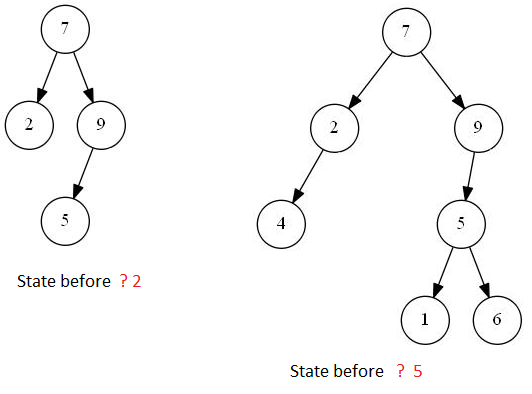
\includegraphics[width=4in]{ex07-aliens/aliens01.png}}
\caption{\label{fig:ex06-basic-shapes} The data structure at two moments in time.}
\end{figure}





\end{document}

